
\begin{figure}
\scriptsize{
\medskip
%%%%%%%%%%%%%%%%%%%%
$
\inferrule
{
}
{P \jp \FH{\phi}{\skipstmt}{\phi}}
\;(\textsc{Skip})
$
\medskip
%%%%%%%%%%%%%%%%%%%%
%% $
%% \inferrule
%% {
%% \mov(P) = \perp
%% }
%% {P \jp \FH{\phi}{\assert{\locExpr}}{\phi}}
%% \;(\textsc{Assert1})
%% $
%% \medskip
%% %%%%%%%%%%%%%%%%%%%%
%% $
%% \inferrule
%% {
%% }
%% {P \jp \FH{\phi \wedge \locExpr}{\assert{\locExpr}}{\phi}}
%% \;(\textsc{Assert2})
%% $
%% \medskip
%%%%%%%%%%%%%%%%%%%%
$
\inferrule
{
}
{P \jp \FH{e}{\yield{e}}{e}}
\;(\textsc{Yield})
$
\medskip
%%%%%%%%%%%%%%%%%%%%
$
\inferrule
{
\phi_1 \wedge \specs(A) \Rightarrow \phi_2
}
{P \jp \FH{\phi_1}{\call{A}}{\phi_2}}
\;(\textsc{Call-Atomic})
$
\medskip
%%%%%%%%%%%%%%%%%%%%
$
\inferrule
{
}
{P \jp \FH{\pre(P')}{\call{P'}}{\post(P')}}
\;(\textsc{Call-Proc})
$
\medskip
%%%%%%%%%%%%%%%%%%%%
$
\inferrule
{
}
{P \jp \FH{\phi \wedge \pre(P')}{\async{P'}}{\phi}}
\;(\textsc{Async})
$
\medskip
%%%%%%%%%%%%%%%%%%%%
$
\inferrule
{
P \jp \FH{\phi_1 \wedge e}{s}{\phi_2}
}
{P \jp \FH{\phi_1 \wedge e}{\ablock{e}{s}}{\phi_2}}
\;(\textsc{Ablock})
$
\medskip
%%%%%%%%%%%%%%%%%%%%
$
\inferrule
{
P \jp \FH{\phi_1}{s_1}{\phi_2} \\ P \jp \FH{\phi_2}{s_2}{\phi_3}
}
{P \jp \FH{\phi_1}{s_1;s_2}{\phi_3}}
\;(\textsc{Seq})
$
\medskip
%%%%%%%%%%%%%%%%%%%%
$
\inferrule
{
P \jp \FH{e \wedge \phi_1}{s_1}{\phi_2} \\ P \jp \FH{\neg e \wedge \phi_1}{s_2}{\phi_2}
}
{P \jp \FH{\phi_1}{\ite{\locExpr}{s_1}{s_2}}{\phi_2}}
\;(\textsc{Ite})
$
\medskip
%%%%%%%%%%%%%%%%%%%%
$
\inferrule
{
P \jp \FH{e \wedge \locExpr}{s}{e} \\ P \jt \while{e,m}{\locExpr}{s}
}
{P \jp \FH{e}{\while{e,m}{\locExpr}{s}}{e \wedge \neg \locExpr}}
\;(\textsc{While})
$
\medskip
%%%%%%%%%%%%%%%%%%%%

}
\caption{Sequential correctness rules}
\label{fig:sequential-correctness}
\end{figure}

\begin{figure}
\scriptsize{
\medskip
%%%%%%%%%%%%%%%%%%%%
$
\inferrule
{
}
{P \jt \FH{\phi}{\skipstmt}{\phi}}
\;(\textsc{Skip})
$
\medskip
%%%%%%%%%%%%%%%%%%%%
%% $
%% \inferrule
%% {
%% }
%% {P \jt \FH{\phi}{\assert{\locExpr}}{\false}}
%% \;(\textsc{Assert})
%% $
%% \medskip
%%%%%%%%%%%%%%%%%%%%
$
\inferrule
{
}
{P \jt \FH{\phi}{\yield{e}}{\false}}
\;(\textsc{Yield})
$
\medskip
%%%%%%%%%%%%%%%%%%%%
$
\inferrule
{
\mov(P') = \perp
}
{P \jt \FH{\phi}{\call{P'}}{\false}}
\;(\textsc{Call1})
$
\medskip
%%%%%%%%%%%%%%%%%%%%
$
\inferrule
{
\mov(P') \neq \perp \\ \phi_1 \wedge \act(P') \Rightarrow \phi_2
}
{P \jt \FH{\phi_1}{\call{P'}}{\phi_2}}
\;(\textsc{Call2})
$
\medskip
%%%%%%%%%%%%%%%%%%%%
$
\inferrule
{
}
{P \jt \FH{\phi}{\async{P'}}{\phi}}
\;(\textsc{Async})
$
\medskip
%%%%%%%%%%%%%%%%%%%%
$
\inferrule
{
P \jt \FH{\phi_1 \wedge e}{s}{\phi_2}
}
{P \jt \FH{\phi_1 \wedge e}{\ablock{e}{s}}{\phi_2}}
\;(\textsc{Ablock})
$
\medskip
%%%%%%%%%%%%%%%%%%%%
$
\inferrule
{
P \jt \FH{\phi_1}{s_1}{\phi_2} \\ P \jt \FH{\phi_2}{s_2}{\phi_3}
}
{P \jt \FH{\phi_1}{s_1;s_2}{\phi_3}}
\;(\textsc{Seq})
$
\medskip
%%%%%%%%%%%%%%%%%%%%
$
\inferrule
{
P \jt \FH{e \wedge \phi_1}{s_1}{\phi_2} \\ P \jt \FH{\neg e \wedge \phi_1}{s_2}{\phi_2}
}
{P \jt \FH{\phi_1}{\ite{\locExpr}{s_1}{s_2}}{\phi_2}}
\;(\textsc{Ite})
$
\medskip
%%%%%%%%%%%%%%%%%%%%
$
\inferrule
{
P \jt \FH{e \wedge \locExpr}{s}{e \wedge m' < m} \\ e \wedge \locExpr \Rightarrow m \geq 0
}
{P \jt \FH{e}{\while{e,m}{\locExpr}{s}}{e \wedge \neg \locExpr}}
\;(\textsc{While})
$
\medskip
%%%%%%%%%%%%%%%%%%%%

}
\caption{Termination correctness rules}
\label{fig:termination-correctness}
\end{figure}

\begin{figure}
\scriptsize{
\medskip
%%%%%%%%%%%%%%%%%%%%
$
\inferrule
{
}
{P \jr \skipstmt : \epsilon}
\;(\textsc{Skip})
$
\medskip
%%%%%%%%%%%%%%%%%%%%
%% $
%% \inferrule
%% {
%% }
%% {P \jr \assert{\locExpr} : \epsilon}
%% \;(\textsc{Assert})
%% $
%% \medskip
%%%%%%%%%%%%%%%%%%%%
$
\inferrule
{
}
{P \jr \yield{e} : \epsilon}
\;(\textsc{Yield})
$
\medskip
%%%%%%%%%%%%%%%%%%%%
$
\inferrule
{
\mov(P') \neq \perp \\ \act(P') \Rightarrow \havoc{H}
}
{P \jr \call{P'} : \epsilon}
\;(\textsc{Call-Loop})
$
\medskip
%%%%%%%%%%%%%%%%%%%%
$
\inferrule
{
\mov(P') \neq \perp \\ \act(P') \Rightarrow \act{P}
}
{P \jr \ablock{e}{s} : A}
\;(\textsc{Call-Action})
$
\medskip
%%%%%%%%%%%%%%%%%%%%
$
\inferrule
{
\mov(P') \neq \perp \\ \act(P') \Rightarrow \havoc{H}
}
{P \jr \async{P'} : \epsilon}
\;(\textsc{Async})
$
\medskip
%%%%%%%%%%%%%%%%%%%%
$
\inferrule
{
\jp \FH{e}{s}{\havoc{H \cup L}}
}
{P \jr \ablock{e}{s} : \epsilon}
\;(\textsc{Ablock-Loop})
$
\medskip
%%%%%%%%%%%%%%%%%%%%
$
\inferrule
{
\jp \FH{e}{s}{\act(P)}
}
{P \jr \ablock{e}{s} : A}
\;(\textsc{Ablock-Action})
$
\medskip
%%%%%%%%%%%%%%%%%%%%
$
\inferrule
{
P \jr s_1 : \re_1 \\ P \jr s_2 : \re_2
}
{P \jr s_1;s_2 : \re_1\cdot\re_2}
\;(\textsc{Seq})
$
\medskip
%%%%%%%%%%%%%%%%%%%%
$
\inferrule
{
P \jr s_1 : \re_1 \\ P \jr s_2 : \re_2
}
{P \jr \ite{\locExpr}{s_1}{s_2} : \re_1+\re_2}
\;(\textsc{Ite})
$
\medskip
%%%%%%%%%%%%%%%%%%%%
$
\inferrule
{
P \jr s : \re
}
{P \jr \while{e,m}{\locExpr}{s} : \re^*}
\;(\textsc{While})
$
\medskip
%%%%%%%%%%%%%%%%%%%%

}
\caption{Refinement rules}
\label{fig:refinement}
\end{figure}


\begin{figure}
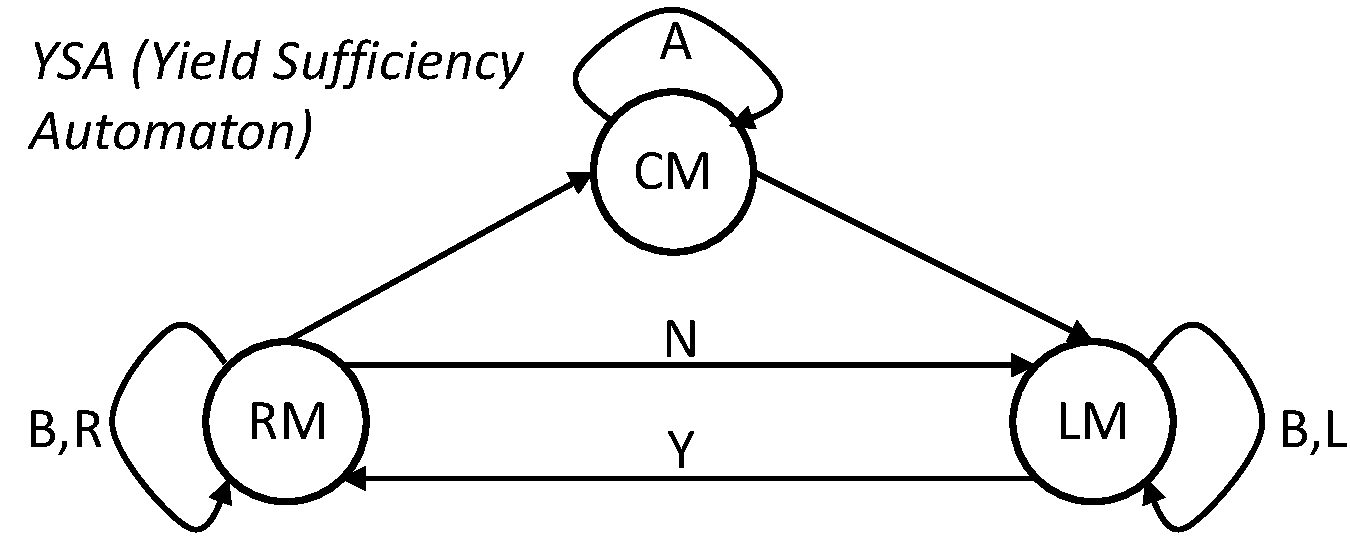
\includegraphics[scale=0.35]{YieldTypeCheckingAutomaton.pdf}
\caption{Specification for yield sufficiency}
\label{fig:YieldTypeCheckingAutomaton}
\end{figure}

\begin{figure}
\scriptsize{
\medskip
%%%%%%%%%%%%%%%%%%%%
$
\inferrule
{
}
{P \jy \skipstmt : x \leadsto x}
\;(\textsc{Skip})
$
\medskip
%%%%%%%%%%%%%%%%%%%%
%% $
%% \inferrule
%% {
%% }
%% {P \jy \assert{\locExpr} : x \leadsto x}
%% \;(\textsc{Assert})
%% $
%% \medskip
%%%%%%%%%%%%%%%%%%%%
$
\inferrule
{
}
{P \jy \yield{e} : x \leadsto \RM}
\;(\textsc{Yield})
$
\medskip
%%%%%%%%%%%%%%%%%%%%
$
\inferrule
{
\mov(P') = B
}
{P \jy \call{P'} : x \leadsto x}
\;(\textsc{CallBothMover})
$
\medskip
%%%%%%%%%%%%%%%%%%%%
$
\inferrule
{
\mov(P') = R
}
{P \jy \call{P'} : \RM \leadsto \RM}
\;(\textsc{CallRightMover})
$
\medskip
%%%%%%%%%%%%%%%%%%%%
$
\inferrule
{
\mov(P') = L
}
{P \jy \call{P'} : x \leadsto \LM}
\;(\textsc{CallLeftMover})
$
\medskip
%%%%%%%%%%%%%%%%%%%%
$
\inferrule
{
\mov(P') = N
}
{P \jy \call{P'} : \RM \leadsto \LM}
\;(\textsc{CallYield})
$
\medskip
%%%%%%%%%%%%%%%%%%%%
$
\inferrule
{
\mov(P') = \perp
}
{P \jy \call{P'} : x \leadsto \RM}
\;(\textsc{CallYield})
$
\medskip
%%%%%%%%%%%%%%%%%%%%
$
\inferrule
{
}
{P \jy \async{P'} : x \leadsto \LM}
\;(\textsc{Async})
$
\medskip
%%%%%%%%%%%%%%%%%%%%
$
\inferrule
{
x \in \{\RM,\CM\}
}
{P \jy \ablock{e}{s} : x \leadsto \CM}
\;(\textsc{Ablock})
$
\medskip
%%%%%%%%%%%%%%%%%%%%
$
\inferrule
{
P \jy s_1 : x \leadsto y \\ P \jy s_2 : y \leadsto z
}
{P \jy s_1;s_2 : x \leadsto z}
\;(\textsc{Seq})
$
\medskip
%%%%%%%%%%%%%%%%%%%%
$
\inferrule
{
P \jy s_1 : x \leadsto y \\ P \jy s_2 : x \leadsto y
}
{P \jy \ite{\locExpr}{s_1}{s_2} : x \leadsto y}
\;(\textsc{Ite})
$
\medskip
%%%%%%%%%%%%%%%%%%%%
$
\inferrule
{
P \jy s : x \leadsto x
}
{P \jy \while{e,m}{\locExpr}{s} : x \leadsto x}
\;(\textsc{While})
$
\medskip
%%%%%%%%%%%%%%%%%%%%

}
\caption{Yield sufficiency rules}
\label{fig:yield-sufficiency}
\end{figure}
